
\section{An \pdfEinfty-structure on cubical chains} \label{s:action}

In this section we construct a natural $\M$-bialgebra structure on the chains of standard cubes.
These are determined by three natural linear maps satisfying the relations defining $\mathcal M$.
A Yoneda extension then provides the chains of any cubical set with a natural $\UM$-coalgebra structure.
We begin by recalling the basics of cubical topology.

\subsection{Cubical sets}

The objects of the \textit{cube category} $\cube$ are the sets $2^n = \{0, 1\}^n$ with $2^0 = \{0\}$ for $n \in \N$, and its morphisms are generated by the \textit{coface} and \textit{codegeneracy} maps
\begin{align*}
\delta_i^\varepsilon & = \mathrm{id}_{2^{i-1}} \times \delta^\varepsilon \times \mathrm{id}_{2^{n-1-i}} \colon 2^{n-1} \to 2^n, \\
\sigma_i & = \mathrm{id}_{2^{i-1}} \times \, \sigma \times \mathrm{id}_{2^{n-i}} \quad \colon 2^{n} \to 2^{n-1},
\end{align*}
where $\varepsilon \in \{0,1\}$ and the functors
\[
\begin{tikzcd} [column sep=16pt]
2^0 \arrow[r, bend left, "\delta^0"] \arrow[r, bend right, "\delta^1"'] & 2^1 \arrow[r, "\sigma"] & 2^0
\end{tikzcd}
\]
are defined by
\[
\delta^0(0) = 0, \qquad \delta^1(0) = 1, \qquad \sigma(0) = \sigma(1) = 0.
\]
We refer to \cite{grandis2003cubical} for a more leisure exposition and for variations on this definition.

We denote by $\cube_{\deg}(2^m, 2^n)$ the subset of morphism in $\cube(2^m, 2^n)$ of the form $\sigma_i \circ \tau$ with $\tau \in \cube(2^m, 2^{n+1})$.

The category of \textit{cubical sets} $\Fun(\cube^\op, \Set)$ is denoted by $\cSet$ and the \textit{standard $n$-cube} $\yoneda(2^n)$ by $\cube^n$.
For any cubical set $X$ we write, as usual, $X_n$ instead of $X(2^n)$.

\subsection{Cubical singular complex}

Consider the topological $n$-cube
\begin{equation} \label{e:topological cube}
\gcube^{n} = \big\{ (x_1, \dots, x_n) \mid x_i \in [0,1] \big\}.
\end{equation}
The assignment $2^n \to \gcube^n$ defines a functor $\cube \to \Top$ with
\begin{align*}
\delta^\varepsilon_i(x_1, \dots, x_n) &= (x_1, \dots, x_i, \varepsilon, x_{i+1}, \dots x_n), \\
\sigma_i(x_1,\dots,x_n) &= (x_1, \dots, \widehat{x}_i, \dots, x_n).
\end{align*}
Its Yoneda extension is known as \textit{geometric realization}.
It has a right adjoint $\cSing \colon \Top \to \cSet$ given by
\[
Z \to \Big(2^n \to \Top(\gcube^n, Z)\Big)
\]
and referred to as the \textit{cubical singular complex} of the topological space $Z$.

\subsection{Cubical chains}

The functor of (\textit{normalized}) \textit{chains} $\chains \colon \cSet \to \Ch$ is the Yoneda extension of the functor $\cube \to \Ch$ defined next.
It assigns to an object $2^n$ the chain complex having in degree $m$ the module
\[
\frac{\k\{\cube(2^m, 2^n)\}}{\k\{\cube_{\deg}(2^m, 2^n)\}}
\]
and differential induced by
\[
\partial (\id_{2^n}) = \sum_{i=1}^{n} \ (-1)^i \
\big(\delta_i^1 - \delta_i^0 \big).
\]
To a morphism $\tau \colon 2^n \to 2^{n^\prime}$ it assigns the chain map
\[
\begin{tikzcd}[row sep=-3pt, column sep=normal,
/tikz/column 1/.append style={anchor=base east},
/tikz/column 2/.append style={anchor=base west}]
\chains(\cube^n)_m \arrow[r] & \chains(\cube^{n^\prime})_m \\
\big( 2^m \to 2^n \big) \arrow[r, mapsto] & \big( 2^m \to 2^n \stackrel{\tau}{\to} 2^{n^\prime} \big).
\end{tikzcd}
\]
The chain complex $\chains(\cube^n)$ is isomorphic to both: $\chains(\cube^1)^{\otimes n}$ and the cellular chains on the topological $n$-cube with its standard CW structure $\gchains(\gcube^n)$.
We use the isomorphism $\chains(\cube^n) \cong \gchains(\gcube^1)^{\otimes n}$ when denoting the elements in the basis of $\chains(\cube^n)$ by $x_1 \otimes \dots \otimes x_n$ with $x_i \in \{[0], [0,1], [1]\}$.

For a topological space $Z$, the chain complex $\chains(\cSing Z)$ is referred to as the \textit{cubical singular chains} of $Z$.

\subsection{Serre coalgebra} \label{ss:serre coalgebra}

We now recall the natural (counital and coassociative) coalgebra structure on cubical chains studied by Cartan and Serre, inducing the cup product in the cohomology of cubical sets.

Using a Yoneda extension, it suffices to equip the chains on standard cubes with a natural coalgebra structure.
For any $n \in \N$, define $\epsilon \colon \chains(\cube^n) \to \k$ by
\[
\epsilon \left( x_1 \otimes \dots \otimes x_d \right) = \epsilon(x_1) \dotsm \epsilon(x_n),
\]
where
\[
\epsilon([0]) = \epsilon([1]) = 1, \qquad \epsilon([0, 1]) = 0,
\]
and $\Delta \colon \chains(\cube^n) \to \chains(\cube^n)^{\otimes 2}$ by
\[
\Delta (x_1 \otimes \dots \otimes x_n) =
\sum \pm \left( x_1^{(1)} \otimes \dots \otimes x_n^{(1)} \right) \otimes
\left( x_1^{(2)} \otimes \dots \otimes x_n^{(2)} \right),
\]
where the sign is determined using the Koszul convention, and we are using Sweedler's notation
\[
\Delta(x_i) = \sum x_i^{(1)} \otimes x_i^{(2)}
\]
for the chain map $\Delta \colon \chains(\cube^1) \to \chains(\cube^1)^{\otimes 2}$ defined by
\[
\Delta([0]) = [0] \otimes [0], \quad \Delta([1]) = [1] \otimes [1], \quad \Delta([0,1]) = [0] \otimes [0,1] + [0,1] \otimes [1].
\]

We remark that, using the canonical isomorphism $\chains(\cube^n) \cong \chains(\cube^1)^{\otimes n}$, the coproduct $\Delta$ can be described as the composition
\[
\begin{tikzcd}
\chains(\cube^1)^{\otimes n} \arrow[r, "\Delta^{\otimes n}"] & \left( \chains(\cube^1)^{\otimes 2} \right)^{\otimes n} \arrow[r, "sh"] & \left( \chains(\cube^1)^{\otimes n} \right)^{\otimes 2}
\end{tikzcd}
\]
where $sh$ is the shuffle map that places tensor factors in odd position first.

\subsection{Degree 1 product}

For $n \in \mathbb{N}$ define the \textit{product} $\ast  \colon \chains(\square^n)^{\otimes 2} \to \chains(\square^n)$ by
\begin{align*}
(x_1 \otimes \dots \otimes x_n) \ast (y_1 \otimes \dots \otimes y_n) =
(-1)^{|x|} \sum_{i=1}^n x_{<i}\, \epsilon(y_{<i}) \otimes x_i \ast y_i \otimes \epsilon(x_{>i}) \, y_{>i},
\end{align*}
where
\begin{align*}
x_{<i} & = x_1 \otimes \dots \otimes x_{i-1}, &
y_{<i} & = y_1 \otimes \dots \otimes y_{i-1}, \\
x_{>i} & = x_{i+1} \otimes \dots \otimes x_n, &
y_{>i} & = y_{i+1} \otimes \dots \otimes y_n,
\end{align*}
with the convention
\[
x_{<1} = y_{<1} = x_{>n} = y_{>n} = 1 \in \Z,
\]
and the only non-zero values of $x_i \ast y_i$ are
\[
\ast([0] \otimes [1]) = [0, 1], \qquad  \ast([1] \otimes [0]) = -[0, 1].
\]

\subsection{An \pdfEinfty-structure on cubical chains} \label{ss:main construction}

The following is the main technical result of this paper.

\begin{lemma} \label{l:cubical chain bialgebra}
	The assignment
	\[
	\counit \mapsto \epsilon, \quad \coproduct \mapsto \Delta, \quad \product \mapsto \ast,
	\]
	induces natural $\mathcal M$-bialgebra structure on $\chains(\square^n)$ for every $n \in \mathbb{N}$ or, equivalently, a functor from the cube category to that of $\M$-bialgebras.
\end{lemma}

The category of bialgebras over a prop is in general not cocomplete, but those of algebras and coalgebras over operads are.
So we have the following result, the main contribution of this paper.

\begin{theorem} \label{t:lift to e infinity coalgebras}
	Composing the functor defined in \cref{l:cubical chain bialgebra} with the forgetful functor $\biAlg_{\M} \to \coAlg_{\UM}$ defines a functor from the cube category to $\coAlg_{\UM}$ whose Yoneda extension endows the chains of a cubical set with a natural $E_\infty$-coalgebra structure extending the Serre coalgebra structure.
\end{theorem}

By linear duality, the same argument can be used to define a natural $E_\infty$-algebra structure on cubical cochains.

\subsection{Cup-$i$ coproducts}

N. Steenrod introduced in \cite{steenrod1947products} operations on the mod~2 cohomology of spaces via an explicit construction of natural maps
\[
\Delta_i \colon \chains(\simplex^n) \to \chains(\simplex^n) \otimes \chains(\simplex^n),
\]
where $\chains(\simplex^n)$ is the complex of chains on the standard $n$ simplex and $\Delta_0$ is the Alexander-Whitney diagonal (\cref{ss:simplicial sets}), such that
\begin{equation} \label{e:cupi homological relations}
(1 + T) \Delta_{i-1} = \partial \circ \Delta_i + \Delta_i \circ \partial
\end{equation}
with coefficients in $\Ftwo$.
These maps, referred to as cup-$i$ coproducts, are combinatorially rich, defining for example the nerve of $n$-categories \cite{medina2020globular} as introduced by Street \cite{street1987orientals}, and admitting an axiomatic characterization \cite{medina2018axiomatic}.

In the cubical case, collections of maps satisfying \eqref{e:cupi homological relations} were defined in \cite{kadeishvili1999coproducts} and \cite{pilarczyk2016cubical}.
It is unclear if these are equivalent.
The formulas used by these authors are analogous to those introduced in \cite{medina2021newformulas} for the simplicial case, a dual yet equivalent version of Steenrod's original description.
By the same methods used in \cite{medina2020globular}, these formulas define a cubical nerve for higher categories, but it remains unclear if either agrees with the one defined by the generalized Gray tensor product.

A new description of maps satisfying \eqref{e:cupi homological relations} can be deduced from our $E_\infty$-structure on cubical chains by considering the action of elements of the form:
\begin{center}
	\documentclass{standalone}
\usepackage{tikz}
\usepackage{amsmath}

\begin{document}
\boxed{
	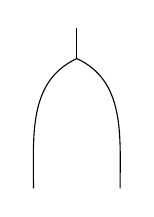
\begin{tikzpicture}[scale=.55]
		\draw (1,3.7) to (1,3);
		\draw (1,3) to [out=205, in=90] (0,0);
		\draw (1,3) to [out=-25, in=90] (2,0);
	\end{tikzpicture}
	\hspace*{1cm}
	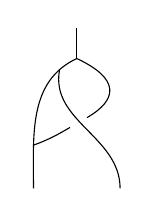
\begin{tikzpicture}[scale=.55]
		\draw (1,3.7) to (1,3);
		\draw (1,3) to [out=205, in=90] (0,0);
		\draw [shorten >= 0cm] (.6,2.73) to [out=-100, in=90] (2,0);
		\draw [shorten >= .15cm] (1,3) to [out=-25, in=30, distance=1.1cm] (1,1.5);
		\draw [shorten <= .1cm] (1,1.5) to [out=210, in=20] (0,1);
	\end{tikzpicture}
	\hspace*{1cm}
	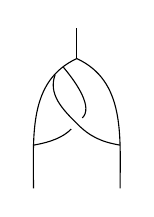
\begin{tikzpicture}[scale=.55]
		\draw (1,3.7) to (1,3);
		\draw (1,3) to [out=205, in=90] (0,0);
		\draw (1,3) to [out=-25, in=90] (2,0);
		\draw [shorten >= 0cm] (.5,2.63) to [out=-110, in=135] (1,1.5);
		\draw [shorten <= 0cm] (1,1.5) to [out=-45, in=170] (2,1);
		\draw [shorten >= .1cm] (.69,2.8) to [out=-50, in=45] (1,1.5);
		\draw [shorten <= .1cm] (1,1.5) to [out=-135, in=10] (0,1);
	\end{tikzpicture}
	\hspace*{1cm}
	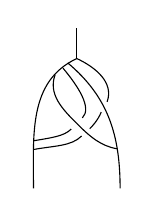
\begin{tikzpicture}[scale=.55]
		\draw (1,3.7) to (1,3);
		\draw (1,3) to [out=205, in=90] (0,0);
		\draw [shorten >= 0cm] (.5,2.63) to [out=-110, in=135] (1,1.5);
		\draw [shorten >= .05cm] (1,1.5) to [out=-45, in=170] (2.02,.9);
		\draw [shorten >= .1cm] (.68,2.78) to [out=-50, in=45] (1,1.5);
		\draw [shorten <= .1cm] (1,1.5) to [out=-135, in=10] (0,1.1);
		\draw (.79,2.9) to [out=-40, in=90] (2,0);
		\draw (1,3) to [out=-25, in=70] (1.7,2);
		\draw [shorten <= .15cm] (1.7,2) to [out=-120, in=45] (1.3,1.38);
		\draw [shorten <= .1cm] (1.24,1.34) to [out=-135, in=10] (0,.9);
	\end{tikzpicture}
}
\end{document}
\end{center}
It is also not known if these agree with either of the previous constructions, pointing to the value of an axiomatic characterization as it exists in the simplicial case, where all known constructions agree.

Cup-$i$ coproducts represent at the chain level Steenrod squares, which are primary operations at the level of cohomology.
To obtain secondary cohomology operations one studies the cohomological relations these operations satisfy, for example the Cartan and Adem relations \cite{steenrod1962cohomology}.
To do this at the cubical chain level, as it was done in \cite{medina2020cartan, medina2021adem} for the simplicial case, the operadic viewpoint is important, so our $E_\infty$-structure on cubical cochains invites the construction of cochain representatives for secondary operations in the cubical case.

For an odd $p$, Steenrod also introduced operations on the mod $p$ cohomology of spaces using the homology of symmetric groups \cite{steenrod1952reduced, steenrod1953cyclic}.
Using the operadic framework of May \cite{may1970general}, we describe in \cite{medina2020maysteenrod} multioperations at the cochain level generalizing the cup-$i$ products in the simplicial and cubical case.

\subsection{Proof of \cref{l:cubical chain bialgebra}} \label{ss:proof action}

We need to show that the assignment
\[
\counit \mapsto \epsilon, \quad \coproduct \mapsto \Delta, \quad \product \mapsto \ast,
\]
is compatible with the relations
\[
\productcounit = 0,
\qquad
\leftcounitality = 0,
\qquad
\rightcounitality = 0,
\]
and
\[
\partial\ \counit = 0,
\hspace*{.6cm}
\partial\ \coproduct = 0,
\hspace*{.6cm}
\partial\ \product = \ \boundary\,.
\]
For the rest of this proof let us consider two basis elements of $\chains(\square^n)$
\begin{align*}
x = x_1 \otimes \dots \otimes x_n
\qquad \text{ and } \qquad
y = y_1 \otimes \dots \otimes y_n.
\end{align*}
Since the degree of $\ast$ is $1$ and $\epsilon([0,1]) = 0$, we can verify the first relation easily:
\begin{align*}
\varepsilon(x \ast y) & =
\sum (-1)^{|x|} \epsilon(y_{<i}) \epsilon(x_{<i}) \otimes \epsilon(x_i \ast y_i) \otimes \epsilon(x_{>i}) \epsilon(y_{>i}) = 0.
\end{align*}
For the second relation we want to show that $(\epsilon \otimes \id) \circ \Delta = \id$.
Since
\begin{gather*}
(\epsilon \otimes \id) \circ \Delta([0]) = \epsilon([0]) \otimes [0] = [0], \qquad
(\epsilon \otimes \id) \circ \Delta([1]) = \epsilon([1]) \otimes [1] = [1], \\
(\epsilon \otimes \id) \circ \Delta([0, 1]) = \epsilon([0]) \otimes [0, 1] + \epsilon([0, 1]) \otimes [1] = [0,1],
\end{gather*}
we have
\begin{align*}
(\epsilon \otimes \id) \circ \Delta (x_1 \otimes \dots \otimes x_n) &=
\sum \pm \left( \epsilon \big(x_1^{(1)}\big) \otimes \dots \otimes \epsilon\big(x_n^{(1)}\big) \right) \otimes
\left( x_1^{(2)} \otimes \dots \otimes x_n^{(2)} \right), \\ &=
x_1 \otimes \dots \otimes x_n,
\end{align*}
where the sign is obtained by noticing that the only non-zero term occurs when each factor $x_i^{(0)}$ is of degree $0$.
The third relation is verified analogously.
The fourth and fifth are precisely the well known facts that $\epsilon$ and $\Delta$ are chain maps.
To verify the sixth and final relation we need to show that
\[
\partial (x \ast y)\ +\ \partial x \ast y\ +\ (-1)^{|x|}x \ast \partial y\ =\ \epsilon(x) y \ -\ \epsilon(y) x.
\]
We have
\[
x \ast y = \sum (-1)^{|x|} x_{<i} \, \epsilon(y_{<i}) \otimes x_i \ast y_i \otimes \epsilon(x_{>i})\, y_{>i}
\]
and
\begin{align*}
\partial(x \ast y) & =
\sum (-1)^{|x|} \, \partial x_{<i}\, \epsilon(y_{<i}) \otimes x_i \ast y_i \otimes \epsilon(x_{>i})\, y_{>i} \\ & +
\sum (-1)^{|x|+|x_{<i}|} \, x_{<i}\, \epsilon(y_{<i}) \otimes \partial (x_i \ast y_i) \otimes \epsilon(x_{>i}) \, y_{>i} \\ & -
\sum (-1)^{|x|+|x_{<i}|} \, x_{<i}\, \epsilon(y_{<i}) \otimes x_i \ast y_i \otimes \epsilon(x_{>i})\, \partial y_{>i}.
\end{align*}
Since
\[
|x| = |x_{<i}| + |x_i| + |x_{>i}|, \quad \epsilon(x_{>i}) \neq 0 \Leftrightarrow |x_{>i}| = 0, \quad \partial(x_i \ast y_i) \neq 0 \Rightarrow |x_i| = 0,
\]
we have
\begin{equation} \label{e:boundary of product 1}
\begin{split}
\partial(x \ast y) & =
\sum (-1)^{|x|} \, \partial x_{<i}\, \epsilon(y_{<i}) \otimes x_i \ast y_i \otimes \epsilon(x_{>i})\, y_{>i} \\ & +
\sum x_{<i} \, \epsilon(y_{<i}) \otimes \partial (x_i \ast y_i) \otimes \epsilon(x_{>i})\, y_{>i} \\ & -
\sum x_{<i} \, \epsilon(y_{<i}) \otimes x_i \ast y_i \otimes \epsilon(x_{>i})\, \partial y_{>i}.
\end{split}
\end{equation}
We also have
\begin{align*}
\partial x \ast y & =
\sum (-1)^{|x|-1} \, \partial x_{<i}\, \epsilon(y_{<i}) \otimes x_i \ast y_i \otimes \epsilon(x_{>i}) \, y_{>i} \\ & +
\sum (-1)^{|x|-1+|x_{<i}|} \, x_{<i}\, \epsilon(y_{<i}) \otimes \partial x_i \ast y_i \otimes \epsilon(x_{>i}) \, y_{>i} \\ & +
\sum (-1)^{|x|-1+|x_{<i}|} \, x_{<i}\, \epsilon(y_{<i}) \otimes x_i \ast y_i \otimes \epsilon(\partial x_{>i}) \, y_{>i}.
\end{align*}
Since
\[
\epsilon(\partial x_{>i}) = 0, \quad \partial x_i \neq 0 \Leftrightarrow |x_i| = 1,
\]
we have
\begin{equation} \label{e:boundary of product 2}
\begin{split}
\partial x \ast y & =
\sum (-1)^{|x|-1} \, \partial x_{<i}\, \epsilon(y_{<i}) \otimes x_i \ast y_i \otimes \epsilon(x_{>i})\, y_{>i} \\ & +
\sum x_{<i}\, \epsilon(y_{<i}) \otimes \partial x_i \ast y_i \otimes \epsilon(x_{>i})\, y_{>i}.
\end{split}
\end{equation}
We also have
\begin{align*}
(-1)^{|x|} \, x \ast \partial y & =
\sum x_{<i} \, \epsilon(\partial y_{<i}) \otimes x_i \ast y_i \otimes \epsilon(x_{>i})\, y_{>i} \\ & +
\sum (-1)^{|y_{<i}|} \, x_{<i}\, \epsilon(y_{<i}) \otimes x_i \ast \partial y_i \otimes \epsilon(x_{>i}) \, y_{>i} \\ & +
\sum (-1)^{|y_{<i}| + |y_i|} \, x_{<i}\, \epsilon(y_{<i}) \otimes x_i \ast y_i \otimes \epsilon(x_{>i}) \, \partial y_{>i},
\end{align*}
which is equivalent to
\begin{equation} \label{e:boundary of product 3}
\begin{split}
(-1)^{|x|} \, x \ast \partial y & =
\sum x_{<i} \, \epsilon(y_{<i}) \otimes x_i \ast \partial y_i \otimes \epsilon(x_{>i})\, y_{>i} \\ & +
\sum x_{<i}\, \epsilon(y_{<i}) \otimes x_i \ast y_i \otimes \epsilon(x_{>i})\, \partial y_{>i}.
\end{split}
\end{equation}
Putting identities \eqref{e:boundary of product 1}, \eqref{e:boundary of product 2} and \eqref{e:boundary of product 3} together, we get
\begin{align*}
\partial (x \otimes y) \ +\ & \partial x \ast y\ +\, (-1)^{|x|}x \ast \partial y \\
& = \sum \epsilon(y_{<i})\, x_{<i} \otimes \big(\partial(x_i \ast y_i) + \partial x_i \ast y_i + x_i \ast \partial y_i\big) \otimes \epsilon(x_{>i})\, y_{>i}.
\end{align*}
Since
\begin{align*}
\partial(x_i \ast y_i)\ +\ \partial x_i \ast y_i\ +\ x_i \ast \partial y_i =
\epsilon(x_i)y_i\ -\ \epsilon(y_i)x_i,
\end{align*}
we have
\begin{align*}
\partial (x \ast y) \ +\ \partial x \ast y\ +\ & (-1)^{|x|}x \ast \partial y \\ = \ &
\sum \epsilon(y_{<i}) \, x_{<i} \otimes \epsilon(x_{\geq i}) y_{\geq i}\ -\
\epsilon(y_{\leq i}) \, x_{\leq i} \otimes \epsilon(x_{>i}) y_{>i} \\ = \ &
\epsilon(x)y - \epsilon(y)x,
\end{align*}
as desired, where the last equality follows from a telescopic sum argument.